\documentclass{article}

% if you need to pass options to natbib, use, e.g.:
% \PassOptionsToPackage{numbers, compress}{natbib}

% ready for submission
\usepackage{aaai}

% to compile a preprint version, e.g., for submission to arXiv, add
% add the [preprint] option:
% \usepackage[preprint]{nips_2018}

% to compile a camera-ready version, add the [final] option, e.g.:
% \usepackage[final]{nips_2018}

% to avoid loading the natbib package, add option nonatbib:
% \usepackage[nonatbib]{nips_2018}

\usepackage[utf8]{inputenc} % allow utf-8 input
\usepackage[T1]{fontenc}    % use 8-bit T1 fonts
\usepackage{hyperref}       % hyperlinks
\usepackage{url}            % simple URL typesetting
\usepackage{booktabs}       % professional-quality tables
\usepackage{amsfonts}       % blackboard math symbols
\usepackage{nicefrac}       % compact symbols for 1/2, etc.
\usepackage{microtype}      % microtypography
\usepackage{amssymb}
\usepackage{natbib}
%% The amsthm package provides extended theorem environments
\usepackage{amsthm}
\usepackage{float}
\usepackage{sgame, tikz} % Game theory packages
\usepackage{caption} 
\usepackage{algorithm,algpseudocode}
\usepackage{makecell}
 \usepackage{multirow}
 \usepackage{graphicx}
\theoremstyle{definition}
\newtheorem{definition}{Definition}[section]
\captionsetup{font=footnotesize}
\bibliographystyle{aaai}




% The \author macro works with any number of authors. There are two
% commands used to separate the names and addresses of multiple
% authors: \And and \AND.
%
% Using \And between authors leaves it to LaTeX to determine where to
% break the lines. Using \AND forces a line break at that point. So,
% if LaTeX puts 3 of 4 authors names on the first line, and the last
% on the second line, try using \AND instead of \And before the third
% author name.




\begin{document}

\title{Competing Bandits}

\author{Guy Aridor\textsuperscript{1}, Kevin Liu\textsuperscript{2}, Aleksandrs Slivkins\textsuperscript{3},
Zhiwei Steven Wu\textsuperscript{4} \\,
{\textsuperscript{1}Columbia University, Department of Economics}\\
{\textsuperscript{2}Columbia University, Department of Computer Science}\\
{\textsuperscript{3}Microsoft Research, New York, NY}\\
{\textsuperscript{4}University of Minnesota - Twin Cities, Department of Computer Science}
}
\maketitle

\begin{abstract}
...
\end{abstract}

\section{Introduction}
\label{intro}

Many modern online platforms simultaneously compete for users as well as learn from the users they manage to attract. For instance, Google Search and Bing compete for users in the search engine market yet at the same need to experiment with their search algorithms to learn what algorithms work the best. This creates a tradeoff between \textit{exploration} and \textit{competition} since firms need to experiment with potentially sub-optimal options for the benefit of gaining information to make better decisions tomorrow while at the same time firms need to incentivize consumers to select them over their competitors today.

From a social welfare perspective it is better for firms to adopt ``smarter" learning algorithms and our main high-level question is asking under what levels of competition are firms incentivized to adopt ``better" learning algorithms. Our primary contribution is that in our model, even in the case of a duopoly, firms are not incentivized to adopt better learning algorithms but that allowing one firm to be a temporary monopolist will incentivize this firm to play a better learning algorithm. 

Unlike in the classic models in economics regarding the interplay between competition and innovation described in \citet{barro2004economic}, here we have no explicit R \& D cost. Rather, firms are not incentivized to experiment under duopoly because experimentation has an implicit relative \textit{reputational} cost compared to the myopic alternative and, in our model, consumers only care about the reputation of a firm. Thus, competition disincentivizes experimentation by firms precisely because competition forces firms to take actions in order to incentivize consumers to select them over their competitors and, as a result, by allowing a firm to be a temporary monopolist the firm can experiment without worrying about the reputational consequences. Our findings give an alternative intuition to the empirically documented inverse-U relationship between competition and innovation discussed in \citet{aghion2005competition}.

\textbf{Related Work} A major underlying component of our model is that firms face a multi-armed bandit (MAB) problem. Multi-armed bandits (MAB) are a tractable abstraction for the tradeoff between exploration and exploitation. MAB problems have been studied for many decades (see \citet{bubeck2012regret} for an overview). Most relevant to this paper is the thread that focuses on designing ``smart" and tractable algorithms that combine exploration and exploitation and ``naive" algorithms that separate exploration and exploitation (see \citet{slivkins2017bandits}).

The three-way tradeoff between exploration, exploitation, and incentives has been studied in several other settings, the most relevant to this paper being \citealt*{che2017recommender}, \citealt*{kremer2014implementing}, \citealt*{mansour2015bayesian}. The strategic experimentation literature in economics, such as \citealt*{bolton1999strategic} and \citealt*{keller2005strategic}, studies models with self-interested agents jointly performing exploration whereas in this paper the firms cannot observe the actions or the payoffs of the other firms and exploration is coordinated by the consumers.

The relationship between competition and innovation has been heavily studied in industrial organization \citep{tirole1988theory} and endogenous growth theory \citep{aghion2005competition, barro2004economic}, dating back to \citet{schumpeter2010capitalism}. 

The most closely related work to this paper is \citealt*{mansour2017competing}. Our motivating questions are the same as \citet{mansour2017competing} though while \citet{mansour2017competing} use the rationality of consumers as their primary knob of competitiveness, we consider differences in the number of firms in the market as our primary knob. Additionally, while in \citet{mansour2017competing} agents select firms based on the Bayesian expected reward of each principal in our model the agents select firms based on a frequentist reputation score that is derived from the signals sent from past agents. This allows the model to become tractable for the purposes of evaluating it via simulation and this is the primary method of analysis that we employ.

\section{Model}
\label{model}

\textbf{Overview} There are two principals and $T+2k$ agents where $k$ is the warm start, or the agents that each principal gets for free at the beginning of the game. The timing of events is as follows:
\begin{enumerate}
\item At $t = 0$, the principals simultaneously commit to following a learning algorithm from a set of algorithms $\mathcal{A}$
\item Still at $t=0$ we suppose that each principal gets $k$ agents as a ``warm" start.
\item A new agent arrives each round (and lives for only one round), starting at $t = 1$, and chooses among 2 principals, given a reputation score for both principals.
\item The principal that is chosen selects an action $a_{t} \in A$ from a set of fixed actions across principals and rounds.
\item Both the agent and the principal observe the reward $r_t \in [0, 1]$ from the action. The agent reports this reward to the principal and the future agents and the reputation score for the chosen principal is updated.
\item Repeat 2-4 for $T$ rounds.
\end{enumerate}

Generally, the rewards are i.i.d. with a common prior.  For computational tractability we restrict our focus to Bernoulli-distributed rewards with Beta priors. Each principal faces a multi-armed bandit problem with no initial information \footnote{For algorithms that require some sort of prior to operate, such as Thompson Sampling, we use a ``fake" prior of $Beta(\alpha=1,\beta=1)$}. We assume that the principals commit to a multi-armed bandit learning algorithm at the start of the world and that there are no informational spillovers from their competitors so that they can only learn from the agents that select them.

\noindent \textbf{Agents} We suppose that agents are myopic and non-strategic. The utility function for the agents is simply to maximize their reward in the one period in which they are alive. We suppose that agents do not attempt to manipulate the strategy of the principal nor do they take the strategies of the principal into account when choosing between the principals. In our model, each agent uses the average reward of past agents as a proxy for their expected utility. For simplicity, the reputation score, $R_jt$ is defined as a sliding window average.
\begin{center}
$R_{jt} = \frac{1}{M} \sum\limits_{i=1}^{M} r_{t_j-i}$
\end{center}

Note that the reputation score is in terms of \textit{local} and not global time so that it is the sliding window average of the last $M$ times that principal $j$ was selected by the agents. The warm start of $k$ rounds allows this reputation score to be well-defined once the ``competition game" begins. In our model the agents deterministically choose the principal with the higher reputation score and ties are broken uniformly at random.

\noindent \textbf{Principals} We suppose that the principals simply care about maximizing market share (i.e. maximizing the number of $T$ agents who select them). We model the ``competition" game between principals as a simultaneous move game where both principals commit to a learning algorithm.

\noindent \textbf{MAB algorithms} We suppose that principals commit to a learning algorithm from $\mathcal{A}$. We partition the set of possible learning algorithms into three different types of learning algorithms and restrict $\mathcal{A}$ to contain a representative each algorithm from each class:
\begin{enumerate}
\item ``Smart" algorithms that engage in adaptive exploration and combine exploration and exploitation. We consider $Thompson Sampling$ (from hereon $TS$) from this class, which, in a given period, will pull an arm according to the probability that that arm is ``optimal" in the sense of having the highest mean reward \citep{agrawal2012analysis}.
\item ``Naive" algorithms that engage in non-adaptive exploration algorithms and separate exploration and exploitation. We consider $Dynamic$ $\epsilon$-$greedy$ (from hereon $DEG$) from this class, which, in a given period, pulls the arms with the highest posterior mean for $1 - \epsilon$ probability and selects a random arm with $\epsilon$ probability. For our experiments we keep $\epsilon = 0.05$ fixed.
\item Greedy / myopic algorithms that engage in no purposeful exploration and take the best short-sighted action. We consider $DynamicGreedy$ (from hereon $DG$) from this class, which, in a given period, pulls the arm with the highest posterior mean.
\end{enumerate}

It is known that $TS > DEG > DG$ in the standard multi-armed bandit problem of minimizing total regret. The primary question that we want to understand is when, in competition, are the principals incentivized to adopt the ``better" algorithms?

\noindent \textbf{Incumbent} In some of our experiments we modify our model so that one principal enters the market $X$ number of rounds before the other. We refer to the principal that enters before as the ``incumbent" and the principal that enters after $X$ rounds as the ``entrant." The agents that arrive in these $X$ rounds are forced to select the only firm in the market as there is no outside option. We treat $X$ as being an exogenous element of the model and study the consequences for a fixed $X$. We have that both the incumbent and entrant commit to a learning algorithm \textit{before} either firm receives any agent. After the $X$ rounds, both firms still receive the $k$ warm start agents.

\section{Simulation Details}
\label{sim_details}

We evaluate the consequences of our model via simulation.

\textbf{Bandit Priors} We look at bandit instances drawn from three different bandit ``priors" that are different types of learning problems. Recall that we only consider Bernoulli-distributed arms and so we draw the true means of the arms from these priors. For these experiments we fix the number of arms we consider, $K = 10$.
\begin{enumerate}
\item Needle In Haystack - $K-1$ arms with mean 0.5 and 1 arm with 0.7.
\item Uniform - the $K$ arms have means drawn uniformly at random from $[0.25, 0.75]$
\item "Heavy Tail" - the $K$ arms have means drawn from $Beta(\alpha=0.6, \beta = 0.6)$. With this prior it was likely to have means at the ``extremes" or means that were close to 0 as well as means that were close to 1.
\end{enumerate} 

\noindent \textbf{Simulation of Competition Game} Unless otherwise noted, all of the reported results utilize the same set of randomly drawn bandit instances and realizations from the prior. Namely, for each bandit prior we draw $N = 1000$ bandit instances. For each of these instances we run simulations of our model for varying values of $k$ and $X$. We take the maximum values of $k$ and $X$ for the simulations we run, $k_{max}$ and $X_{max}$ respectively, and compute a realization table of dimension $(T+k_{max}+X_{max}) \times K$. 

This realization table, as well as fixing the random seed for the same bandit instance and realization table across experiments, ensures that differences in algorithm performance are not due to noise in the realizations but due to differences in the algorithms in the different experimental settings. In the competition game we draw from the $T \times K$ portion of the table, so that if two different algorithms picks arm $a$ at time $t$, they get the same $[a, t]$ realization in the table. This setup also ensures that in the warm start period, increasing the warm start from $k$ to $k + 10$ results in the same behavior in the first $k$ rounds.

For the simulations we fix the sliding window size $M = 100$. Low values of $M$ induced too much random noise into the results and we found that increasing $M$ to be larger than $100$ did not make a substantial qualitative difference so we fix this value.

\section{Performance in Isolation}
\label{iso_section}

We evaluate the performance of the different learning algorithms on the bandit priors we consider in isolation. There are two reasons why this is important to consider. First, we want to confirm that the reputation ordering of the algorithms is what we would expect according to the multi-armed bandit literature where $TS > DEG > DG$. Second, we want to better understand what statistics of the instance we can look at in isolation in order to help us predict and understand what to expect in the competition game.

\begin{figure}
\caption{Mean Reputation Trajectories in Isolation}
\includegraphics[scale=0.25]{"figures/nih_iso_mean"}
\label{prelim_means}
\caption*{\tiny{The plots contain the average reputation over $1000$ runs for a memory size of $100$ where, for a given $t$, we record the reputation of a given algorithm on a given instance and then average this value across all the runs. The shaded area display 95\% confidence intervals.}}
\end{figure}

Figure \ref{prelim_means} shows that the mean reputation ordering is as we would expect for the Needle In Haystack prior. The mean reputation ordering that we expect also holds for the other two priors and the results for those can be found in the GitHub appendix.

In the ``competition" game the agents decide between the principals using the \textit{relative} reputation between the two principals. Namely, if principal $A$ has a higher reputation than principal $B$ agents will select principal $A$. A natural question to ask is whether looking at the mean performance is sufficient for understanding performance in the competition game. Figure \ref{rep_dist_nih} displays the reputation distribution at $t = 500$ for the same prior we reported the mean plot for previously. We see that the ``naive" algorithms $DG$ and $DEG$ have a bi-modal reputation distribution whereas $TS$ does not. The intuition for this is that, for Needle In Haystack, $DG$ either finds the best arm or not. If it does, then since it engages in no purposeful exploration it will do better than any algorithm that engages in purposeful exploration over sufficiently many rounds so that the weak law of large numbers comes into play (our $M$ is set sufficiently high to ensure this most of the time). However, if it does not then it will get stuck on a bad arm and lose to $TS$ or $DEG$. In these cases its reputation may be substantially worse but for the competition game the difference between the reputation does not matter but only the binary comparison between them \footnote{This holds for our model and the decision rule of the agents, though the absolute difference may matter if, for instance, considering the SoftMax decision rule in \citet{mansour2017competing}}.

\begin{figure}
\caption{Reputation Distribution}
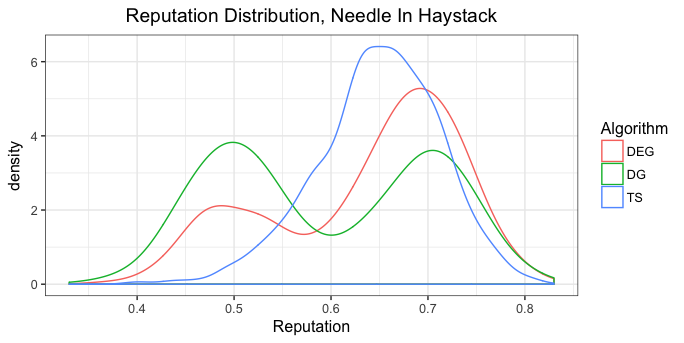
\includegraphics[scale=0.3]{figures/rep_distribution_nih}
\label{rep_dist_nih}
\caption*{\tiny{The plots contain a kernel density estimate of the reputation distribution at $t = 200$}}
\end{figure}

This motivates looking at the entire distribution of reputation difference between two algorithms. Figure \ref{ts_dg_rep_diff_nih} shows the distribution of reputation difference between $TS$ and $DG$ across $t$. This figure seems to confirm the intuition noted previously since the reputation distribution has its largest mass around the point just below 0 but it is skewed to the right. Thus, the mean is not a representative statistic of the entire reputation difference distribution. As an alternative statistic for understanding the results of the competition game we introduce the \textit{relative reputation statistic} which looks at the proportion of simulations in which algorithm $A$ had at least as high of a reputation as algorithm $B$ for a fixed time $t$. This corresponds to running the bandit algorithms in isolation on the same instance and with the same realizations for $t$ rounds and then calculating the fraction of simulations at which an agent would select a principal playing $A$ over a principal playing $B$ at time $t$ \footnote{Though we do not discuss it here, one may be interested in if there is ever a case where, for sufficiently large $t$, we observe that $DEG >DG$ or $TS > DG$ according to the mean reputation but $DG > DEG$ or $DG > TS$ according to the relative reputation proportion. In the GitHub appendix we have results showing that, for Heavy Tail prior with $K=3$ we have that $DEG > DG$ according to the mean reputation but $DG > DEG$ according to the relative reputation proportion.}.

\begin{figure}
\caption{Reputation Difference Distribution}
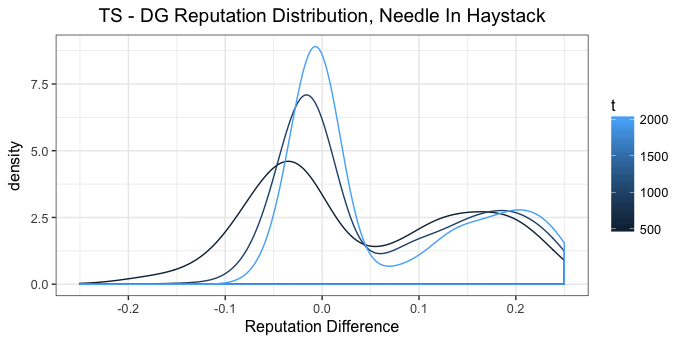
\includegraphics[scale=0.3]{figures/ts_dg_rep_diff_nih}
\label{ts_dg_rep_diff_nih}
\caption*{\tiny{The plots contain a kernel density estimate of the difference in reputation between $TS$ and $DG$ across $t$}}
\end{figure}


\begin{figure}
\caption{Relative Reputation Plots}
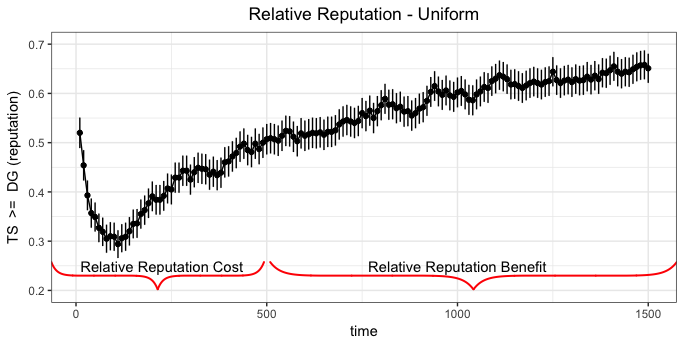
\includegraphics[scale=0.35]{figures/relative_uniform_annotated_plot}
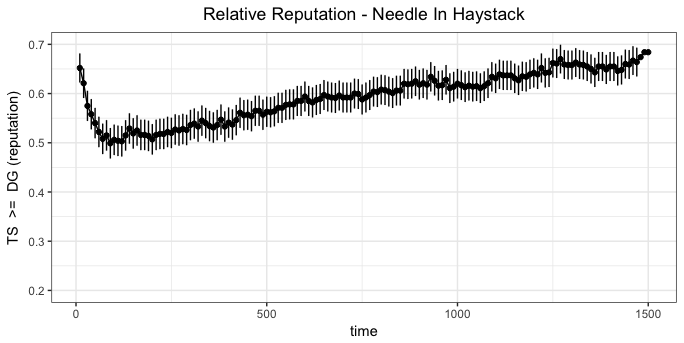
\includegraphics[scale=0.35]{figures/ts_dg_nih_10_prelim}
\caption*{The plots contain the average reputation over $1000$ runs for a memory size of $100$ where, for a given $t$, we record the reputation of both of the algorithms on a given instance and then calculate the proportion of runs where $TS \geq DG$. The shaded area display 95\% confidence intervals.}
\label{relative_rep_plots}

\end{figure}

Figure \ref{relative_rep_plots} shows the relative reputation plots for $TS$ vs $DG$ on the Uniform and Needle In Haystack prior. For the Uniform prior we see that, in the early rounds, $DG > TS$ for the majority of the simulations but that, eventually, $TS > DG$. The intuition behind this is that, especially since the principals start with no substantive initial information, $TS$ does purposeful exploration in the early rounds in order to acquire information. However, this exploration leads to what we define as a \textit{relative reputation cost}. Namely, exploration leads to lower reputation relative to the myopic alternative. However, eventually the information acquired in the early rounds allows $TS$ to make better decisions and achieve a higher reputation, especially when the instance is ``hard enough" so that $DG$ cannot trivially find the best arm. We define this as the \textit{relative reputation benefit} \footnote{We see similar behavior for the Heavy Tail prior}.

Is exploration always costly? Figure \ref{relative_rep_plots} also shows that for the Needle In Haystack prior, $TS$ always does relatively better than $DG$. There are two contributing factors to this. First, $TS$ identifies the best arm faster in the Needle In Haystack prior than the Uniform prior so that there is a shorter time horizon where $TS$ needs to engage in purposeful exploration. Second, in the Needle In Haystack prior there are no ``bad" arms as there may be in the Uniform prior since by construction all the arms except one in Needle In Haystack are the same. Thus, when $TS$ pulls a sub-optimal arm relative to its current information, the expected reward is the same as the greedy option that has not identified the best arm. However, with the Uniform prior, it is possible that the sub-optimal arm that is pulled has substantially lower expected reward relative to the greedy option.

\section{Monopoly vs Duopoly}

In this section we utilize the same instances and realizations as in the previous section and simulate the model described in section \ref{model}. We initially take the strategies of the firms as exogenous and simulate the model given these strategies in order to determine the payoffs associated with each pair of algorithms. Unless otherwise noted, all the results are reported at $t = 2000$.






\bibliography{refs}

\end{document}
